% =====================================================================
% A Lock-Free Data Plane and the Signal-to-Seed Bottleneck in Nanopore
% Adaptive Sampling
%
% Springer LNCS proceedings format (llncs.cls), converted from the
% IEEEtran version by scripts/make_springer_manuscript.py. Body text is
% identical to that version; edit paper/manuscript-ieee.tex and
% regenerate rather than editing this file.
%
% ABRIDGED TO 12 PAGES for a venue with that limit. The IEEE version
% is the full paper; the units cut here are listed, with reasons, in
% scripts/make_springer_manuscript.py.
%
% TODO BEFORE SUBMISSION
%   1. ORCID iDs: append \orcidID{...} after each name in \author if you
%      have them. Springer encourages these.
%
% IF THE VENUE PUBLISHES IN A DIFFERENT SPRINGER SERIES
%   LNCS, CCIS and LNNS all use llncs.cls, so nothing below changes.
%   Only LNEE or a Springer Nature journal template would alter the
%   class line; the body is unaffected either way.
%
% FIGURES expected in ./figures/ :
%   fig7-3-model-vs-measured.pdf     (the only figure in this version)
% =====================================================================
\documentclass[runningheads]{llncs}

\usepackage[utf8]{inputenc}
\usepackage[T1]{fontenc}
\usepackage{amsmath,amssymb}
\usepackage{graphicx}
\usepackage{booktabs}
\usepackage{textcomp}
\usepackage{url}

\graphicspath{{figures/}}
\renewcommand{\arraystretch}{1.15}

% Long unbreakable technical tokens -- script paths, chains of \times in maths -- can leave
% a line with nowhere to break. Letting TeX stretch the interword space on such a line keeps
% them out of the margin without touching a word.
\emergencystretch=1.5em

\begin{document}

\title{A Lock-Free Data Plane and the Signal-to-Seed Bottleneck in
Nanopore Adaptive Sampling}

% Shortened form for the running head, as llncs requires for long titles.
\titlerunning{A Lock-Free Data Plane and the Signal-to-Seed Bottleneck}

% To add ORCIDs, append \orcidID{0000-0000-0000-0000} after each name.
\author{Khushal Singh\inst{1} \and Ritu Garg\inst{1}}
\authorrunning{K. Singh and R. Garg}

\institute{Department of Computer Engineering, National Institute of
Technology Kurukshetra, Kurukshetra, Haryana 136119, India\\
\email{khushal6002@gmail.com}, \email{ritu.59@nitkkr.ac.in}}

\maketitle

\begin{abstract}
Oxford Nanopore adaptive sampling (``Read Until'') requires a client to
decide, within a physical deadline, whether to eject a molecule still transiting the pore.
First, the decision budget is not the obstacle: a single-process C++20 data plane with
single-copy ingestion, zero-copy propagation and a lock-free, reference-counting arena
protocol reaches a median per-chunk decision latency of 124.8 \textmu{}s [115.6--132.3] against a
derived service bound of 1.56 ms, with no drops at genome scale. A basecalling client's bare
orchestration (readfish with a no-operation caller) costs 124.3 \textmu{}s per read-chunk on the same
rig---as much as our \emph{complete} signal-space decision. Read Until is a soft-real-time
\emph{loss system}: a mean inside budget is consistent with an arbitrary deadline-miss rate.
Second, we locate the real limit. Our pipeline resolves 17.6\% [16.6--18.8] of reads at a
zero-false-positive threshold where RawHash2 resolves 91.8\% [91.2--92.4] on identical
input. We proposed a seed-survival law
$P(\mathrm{key}) = a^{E}$ in per-event bucket agreement $a$ and key length $E$, argued it was
a lower bound, and then \emph{refuted our own bound}: once event retention is data-dependent
the form is $P(\mathrm{key}) \approx (1-g)^{E} a^{E}$, where $g$ is the correspondence-failure
rate. Under one estimator, RawHash2 achieves $a = 0.911$, $g = 0.092$ and
467 anchors per read at $E = 8$, against our 0.783, 0.196 and 14.9 at $E = 12$. We trace this
to three causes, each of which we measure: the two encoders retain events asymmetrically, the
quantiser buys too little agreement, and the chainer loses recoverable anchors.

\keywords{nanopore sequencing \and adaptive sampling \and soft real-time systems \and lock-free data structures \and raw signal mapping \and quantisation}
\end{abstract}

\section{Introduction}
\label{sec:intro}

Nanopore sequencing reads a molecule as it passes through a pore, recording the resulting ionic
current in real time. Because the signal arrives while the molecule is still in the pore, the
instrument exposes an interface, Read Until, through which a client can request that an
unwanted molecule be ejected and the channel freed for another. The benefit is a higher
on-target yield with no change to library preparation.

Read Until imposes a deadline, and that deadline is physical rather than conventional. Signal
is delivered in fixed-rate chunks, each describing bases that have \emph{already} passed
through the pore. A decision that arrives after the molecule has left is not merely late; it is
worthless. Let $C$ be the number of active channels, $T_c$ the interval between chunks on one
channel, and $W$ the number of chunks after which a decision loses its value. The mean service
time available per decision is then
\begin{equation}
S < \frac{W \cdot T_c}{C},
\label{eq:budget}
\end{equation}
which at $W = 2$, $C = 512$ and $T_c = 0.4$ s gives 1.5625 ms, hereafter 1.56 ms.

The deadline has two consequences for how the problem should be framed, and the paper is
organised around them.

\textbf{Soft real time.} A decision does not lose value gradually; its usefulness falls to zero
at the deadline. The quantity of interest is therefore the \emph{distribution} of decision
latency, not its mean.

\textbf{A loss system, not a delay system.} Under saturation, a client must either queue work or
discard it. Queueing turns decisions that would have been useful into decisions that arrive too
late, so dropping work is the correct policy, not merely a pragmatic one. The
consequence for evaluation is sharp and, we argue, under-appreciated: \textbf{a mean
comfortably inside the budget is consistent with an arbitrary deadline-miss rate.} A system
reporting ``mean 124 \textmu{}s against a 1.56 ms budget'' has said nothing about whether it meets its
deadline.

Existing Read Until work does report latency, in two forms: signal consumed before a decision
(mean bases or chunks per read), and mean processing time per read. What we did not find in the
systems we surveyed is a deadline-miss rate against a stated service bound, a latency
distribution with tail percentiles, or the fraction of decisions arriving too late to act on.
That gap---reporting a distribution against a derived budget, with the instrument and
environment characterised well enough for the tail to carry meaning---motivates the first half
of this paper.

\textbf{Contributions.}
\begin{enumerate}
\item A lock-free soft-real-time data plane for signal-space adaptive sampling, with a
reference-counting arena protocol that makes reset-under-dispatch unrepresentable by
construction rather than by a timing assumption (Section~\ref{sec:plane}), evaluated as a
distribution against a derived budget over nine runs (Section~\ref{sec:eval}).
\item A negative result, explained rather than excused: our pipeline is $5.2\times$ less accurate
than a published signal-space mapper on identical input, and we locate the cause before
seeding (Section~\ref{sec:gap}).
\item A seed-survival law, including the refutation of our own earlier formulation of it, and
an estimator-symmetric measurement of its two parameters for both systems
(Section~\ref{sec:law}).
\item Three measured root causes and the design prescriptions that follow
(Section~\ref{sec:causes}).
\end{enumerate}

\section{Background and related work}

\textbf{The interface.} MinKNOW~\cite{minknow} provides Read Until through a bidirectional
streaming RPC. The client receives raw signal chunks from each channel and sends its decisions
back over the same connection.

\textbf{Basecalling clients.} readfish~\cite{readfish} and similar clients basecall each chunk
and map the resulting sequence. The approach is accurate and builds on mature tools, but it
places both a neural network and a sequence aligner~\cite{minimap2} inside the decision loop.

\textbf{Signal-space mappers} skip basecalling. They use a pore model to convert the reference
into the signal it is expected to produce, and then match quantised query events against it
directly. UNCALLED~\cite{uncalled} builds an FM-index over events. Sigmap~\cite{sigmap} and
RawHash~\cite{rawhash} seed and chain over quantised event $k$-mers. RawHash2~\cite{rawhash2}
extends this with an adaptive quantiser, and RawAlign~\cite{rawalign} adds alignment on top of
seeding. Sigmoni~\cite{sigmoni} classifies reads with an $r$-index over a small picoamp
alphabet. The recent benchmarking framework RawBench~\cite{rawbench} divides raw signal
analysis into reference encoding, segmentation and matching, and evaluates three segmentation
methods: t-test changepoint detection, basecaller move tables and a learned segmenter. We use
the same division, but we split matching further into quantisation, seeding and chaining,
because our argument needs that level of detail.

\textbf{The pipeline is ordered, and earlier stages bound later ones.} The stages are applied in
a fixed order: reference encoding $\rightarrow$ segmentation $\rightarrow$ quantisation
$\rightarrow$ seeding $\rightarrow$ chaining. Each stage sets an upper limit on what the later
stages can achieve. For example, information lost during quantisation cannot be recovered by any
chaining strategy. Sections~\ref{sec:gap}--\ref{sec:causes} follow this order.

\textbf{Streaming decision structures.} Misra--Gries~\cite{misragries} and
Space-Saving~\cite{spacesaving} identify frequent items approximately, using a fixed amount of
memory. We use a set-associative variant as a vote table. Its update cost is $O(\text{ways})$ rather than
$O(\text{counters})$, which is significant on a latency-critical decision path.

\textbf{Simulation.} Squigulator~\cite{squigulator} generates signal with an adjustable spread
of dwell times; its default coefficient of variation (CV) is about 0.44. Icarust~\cite{icarust}
serves a live Read Until API, but it produces the same number of samples for every $k$-mer,
which corresponds exactly to CV $= 0$. We modified Icarust to draw dwell times from a lognormal
distribution.

\section{The data plane}
\label{sec:plane}

\subsection{Design constraints}

The design follows from four constraints.
\begin{enumerate}
\item \emph{No allocation on the decision path.} The time an allocation takes has no upper
bound.
\item \emph{No locks.} A blocked worker still holds a deadline, and it cannot meet it.
\item \emph{State bounded by channel count.} State is $O(\text{channels})$, with per-channel
constants fixed at compile time, because read length is set by library preparation and cannot
be known in advance.
\item \emph{Drop rather than queue.} Under backpressure the system discards work instead of
queueing it, for the loss-system reason given in Section~\ref{sec:intro}.
\end{enumerate}

\subsection{Single-copy ingestion, zero-copy propagation}

The signal is copied only once, at the transport boundary, where the protobuf runtime writes it
into arena-backed storage. After that point, no stage copies the signal again.

\subsection{The arena reference-counting protocol}

The hazard is reset-under-dispatch: an arena slot recycled while a descriptor referring to it
is still in a ring. Because the memory remains mapped and arena-owned, the failure is silent
payload corruption rather than a crash.

The protocol removes it structurally. \texttt{acquire()} returns a
slot at refcount 1, and that initial reference is held by the \textbf{reader}, not by a
consumer. The reader pushes descriptors to $n$ shard rings, raising the count to $1 + n$, and
only then releases its own. The count can therefore reach zero only after every worker
reference has been taken and dropped, and the slot cannot be reset while any dispatch is
outstanding. No bound on how long a worker takes is required.

\subsection{Lock-free handoff and sharding}

Handoff uses single-producer single-consumer rings with free-running 64-bit counters and
power-of-two capacity, so the index is a mask rather than a modulus and the full capacity is
usable rather than capacity $-\,1$. Producer and consumer each cache the other's index,
removing cross-core loads from the unsaturated steady state; head, tail and both cached copies
are separately cacheline-aligned. Shard rings hold 2048 descriptors; action rings hold 1024. At
four shards the rings total under 0.75 MB, negligible beside the index.

Chunks are sharded by \texttt{channel \& mask}, so all per-channel state is reached by exactly
one thread \textbf{by construction}. This is what makes the lock-free claim cheap: there is no
shared mutable per-channel state to protect. Backpressure is drop-never-block, with the
invariant $\textit{offered} = \textit{pushed} + \textit{dropped}$ maintained by counters.

\section{Evaluation of the data plane}
\label{sec:eval}

\subsection{Method and instrumentation}

Latency is the interval from the transport read returning to the decision being reached,
recorded with HdrHistogram~\cite{hdrhistogram} at three significant figures, bounding relative
error at 0.1\%. The recorder reports its own backend on every line, so a degraded estimate
cannot be mistaken for a measurement.

\textbf{Host.} Intel Core i5-1135G7, 4 physical cores / 8 logical, under WSL2.
\textbf{Regime.} R3: a 64 Mb human chr20 reference
under variable dwell at the frozen configuration---4 bits $\times$ 12 events,
minimizer~\cite{minimizers} window
1, detected-event segmentation, two shards, pinned.

\subsection{Genome scale: regime R3}

We made nine runs of 40 s each. In every log, the line the daemon prints at startup confirms the
configuration: 63,981,237 reference bases, a geometry of $4 \times 12 = 48$-bit keys, window 1,
63,981,218 minimizers, 32,888,127 distinct keys, and a 512.0 MiB table plus 204.3 MiB of
positions.

\begin{table}[t]
\caption{Regime R3, nine runs. Median across runs, with observed range, \textmu{}s.}
\label{tab:r3}
\centering
\footnotesize
\begin{tabular}{lr}
\toprule
percentile & median [range] \\
\midrule
p50   & 124.8 [115.6--132.3] \\
p90   & 192.8 [183.0--306.0] \\
p99   & 370.2 [346.8--1969.3] \\
p99.9 & 1224.5 [1044.9--3284.0] \\
mean  & 138.2 [131.2--206.0] \\
\bottomrule
\end{tabular}
\end{table}

Peak resident set is 3.70 GiB in every run---the maximum including the index-build transient;
the steady-state index structures are 716 MiB. Offered chunk arrival is 604--645 per second, set
by the simulator rather than the daemon. \textbf{No chunks were dropped and no deadline misses
were recorded in any of the nine runs.}

At the median this is a utilisation of \textbf{0.080} against the 1.56 ms bound. A 10-chunk read
completes its decisions in \textbf{1.25 ms}---a derivation, ten chunks times the measured median
per-chunk latency, not an independent measurement.

\textbf{The tail is where the loss-system framing earns its place.} Eight of the nine runs sit
strictly inside the budget through the 99.9th percentile, at 1.04--1.40 ms. The ninth does not:
one run reports p99 $=$ 1969.3 \textmu{}s and p99.9 $=$ 3284.0 \textmu{}s, and is also the worst of the nine at
p90 and at the mean.

We do not read this as a deadline miss. Across the nine runs the observed \emph{maximum} spans
2.0 ms to 59.4 ms---two orders of magnitude in a quantity the software should not vary in---and,
tellingly, the run with the largest maximum is \textbf{not} the run with the worst p99; its p99
is 630 \textmu{}s. Maximum and p99 are not correlated here, which is the signature of externally
injected stalls rather than of slow decisions. On a hypervisor without core isolation, this
measurement cannot establish that the system meets its deadline, and cannot establish that it
misses it. Stating that honestly is part of the contribution.

\subsection{Comparison with existing clients}

\begin{table}[t]
\caption{Cost comparison on the same host. readfish figures are its own progress line divided
out; processor and memory figures are from \texttt{/usr/bin/time -v}.}
\label{tab:costs}
\centering
\scriptsize
\begin{tabular}{llrrr}
\toprule
system & mode & per chunk & CPU & peak RSS \\
\midrule
readfish  & no-op caller      & 124.3 \textmu{}s & 15.6\%  & 86.0 MiB \\
readfish  & caller + mapper   & 66.2 \textmu{}s  & 25.3\%  & 663.4 MiB \\
this work & frozen, 64 Mb     & 124.8 \textmu{}s & 181.5--202.3\% & 3786 MiB \\
\bottomrule
\end{tabular}
\end{table}

\textbf{The architectural point.} readfish~\cite{readfish} with a no-operation caller
performs no basecalling
and no mapping; 124.3 \textmu{}s is its orchestration alone, a lower bound on its cost. Our
\emph{complete} signal-space decision over a 64 Mb index costs 124.8 \textmu{}s. The orchestration layer
of a basecalling client is already as expensive as an entire signal-space decision. This does
not establish superiority---a production readfish does work this configuration omits---but it
does establish that the decision budget is not what stands between signal-space matching and
deployment.

The cost is processor time: 181.5--202.3\% of one core against readfish's 15.6\%, because
workers spin before yielding. We report it alongside.

\section{The accuracy gap}
\label{sec:gap}

\subsection{Head-to-head}

Both systems were run on the same 20 Mb chr20 reference, the same
Squigulator~\cite{squigulator}-derived R10.4
9-mer pore model on both sides, the same SLOW5 files, three seeds, 500 reads per cell, at
Squigulator's default dwell dispersion.

Our figures are true-positive rates at the lowest threshold giving zero false positives on a
composition-matched shuffled control. RawHash2's are correctly-mapped fractions at its own
default operating point, which is \textbf{not} zero-false-positive: 8.4--10.6\% of control reads
are mapped. The comparison is of magnitude, not of level, and we state it as such.

\begin{table}[t]
\caption{Accuracy, three seeds, 500 reads per cell.}
\label{tab:acc}
\centering
\footnotesize
\begin{tabular}{lrrrr}
\toprule
system & s42 & s43 & s44 & mean [range] \\
\midrule
this work  & 18.8 & 17.4 & 16.6 & \textbf{17.6} [16.6--18.8] \\
RawHash2   & 92.4 & 91.8 & 91.2 & \textbf{91.8} [91.2--92.4] \\
\bottomrule
\end{tabular}
\end{table}

A factor of 5.2 (Table~\ref{tab:acc}). The rest of this paper accounts for it.

\subsection{Replication is not optional at this scale}

Six decision rules were each run in triplicate at the same operating point.

\textbf{The $\beta = 0$ control is the informative case.} With gap tolerance removed, chaining is
\emph{worse} than the vote table---9.1\% against 14.1\%---as expected when it tracks 24
candidates where the table tracks 256. The improvement is therefore attributable to the
tolerance, not to the change of data structure.

\textbf{The best decision rule is $+35\%$ relative over voting}, 19.0\% against 14.1\%. No rule
we tried exceeded that.

\textbf{Single rules vary by up to 3.8 points across seeds}---the control spans 7.0 to
10.8---comparable to the gaps \emph{between} rules, and the ranges of adjacent rules overlap. Any
comparison between configurations differing by less than roughly four points requires
replication.

Even at its best, the decision rule moves accuracy by tens of percent where the gap to be closed
is a factor of five. The deficiency is not here.

\section{A seed-survival law}
\label{sec:law}

\subsection{The model, and the refutation of our own bound}

Let $a$ be the probability that reference and query assign the same quantiser bucket to
corresponding events. A key packs $E$ consecutive events, so a key matches only if all $E$
agree, and expected anchor yield falls as $a^{E}$.

We originally argued this was a \textbf{lower} bound. Two things make per-event agreements
positively correlated. Consecutive events come from overlapping $k$-mers (two adjacent 9-mers
share eight bases). In addition, all events of a read are normalised with one shift-and-scale
estimate, so an error in that estimate moves all of the read's $z$-values together. When
agreements are positively correlated they tend to cluster, and a run of $E$ events is then more
likely to agree completely than it would be if events were independent.

\textbf{However, this argument depends on a condition that fails for most of the configurations
we study.} It assumes that reference and query events correspond one-to-one. A single inserted
or deleted event in a key window prevents a match, however well the other events agree. Let $g$
be the probability that an alignment column is an indel rather than a matched pair. The
key-match probability is then
\begin{equation}
P(\mathrm{key}) \approx (1-g)^{E} \cdot a^{E},
\label{eq:pkey}
\end{equation}
where the first factor is missing from the simple form. With fixed-width segmentation and
constant dwell, $g$ is small and $a^{E}$ is the lower bound argued above; the direct count
exceeds it by $1.8\times$ and $5.1\times$ in the two such configurations. With data-dependent
segmentation or variable dwell, $g$ rises to 0.09--0.21 and $a^{E}$ becomes an
\textbf{over-estimate}, by $1.9\times$ to $14\times$ across the remaining cells
(Figure~\ref{fig:modelmeas}).

The qualitative content survives---yield falls geometrically in $E$, with a base that is a
measurable property of the quantiser---but the use of $a^{E}$ as a one-sided bound is restricted
to the exact-correspondence case.

\subsection{An estimator-symmetric instrument}

An agreement figure computed two different ways for two systems is not a comparison. We
therefore emit per-event quantised symbols from both systems in one format and score them with
one program, which does not know which system produced its input.

Our symbols come from the production reference-encoding and quantisation paths.
RawHash2~\cite{rawhash2} ships
\texttt{--out-quantize}, which dumps query-side symbols; its reference path hardcodes the dump
off, so we added a four-line \texttt{--out-quantize-ref} exposing the same facility on the
reference side, and fixed a record-separator defect that makes the stock multi-read output
unparseable.

The scorer aligns the two symbol streams semi-globally. The query is aligned in full, end gaps
on the reference are free, and the scores are $+1$ for a match, $-1$ for a mismatch and $-1$
for a gap. It reports $a$ under the maximising alignment, $a$ under the single best constant
offset, the indel fraction, and the fraction of positions that begin a gap-free, all-matching
run of $E$ columns, read directly from the alignment path. This last figure is
$P(\mathrm{key})$ \textbf{measured rather than modelled}, so the independence assumption is no
longer needed at all.

\subsection{Results}

\begin{table}[t]
\caption{Agreement, correspondence failure, and measured key-match probability. 200 reads per
cell, identical input, one estimator.}
\label{tab:agree}
\centering
\scriptsize
\begin{tabular}{llrrrrr}
\toprule
system & CV & $a$ & $g$ & $E$ & $P(\mathrm{key})$ & anchors \\
\midrule
this work & 0.00 & 0.797 & 0.170 & 12 & 0.0124 & 33.8 \\
this work & 0.44 & 0.783 & 0.196 & 12 & 0.0055 & 14.9 \\
RawHash2  & 0.00 & 0.913 & 0.055 & 8  & 0.350  & 651 \\
RawHash2  & 0.44 & 0.911 & 0.092 & 8  & 0.254  & 467 \\
\bottomrule
\end{tabular}
\end{table}

\textbf{The gap is large and it is before seeding.} At CV 0.44, measured key-match probability
differs by a factor of \textbf{46} (0.254 against 0.0055) and anchor supply by a factor of
\textbf{31} (467 against 14.9 per read, the two ratios differing because the systems retain
different numbers of events per read; Table~\ref{tab:agree}). A 31-fold
difference in anchor supply accounts for 91.8\% against 17.6\% without any appeal to the
decision rule.

\textbf{The key-match difference decomposes, and key length is the smaller lever.} Within our
pipeline, measured $P(\mathrm{key})$ at $E = 8$ rather than 12 is 0.0274 against 0.0055, a
factor of \textbf{4.9}. The remaining factor of \textbf{9.3} (0.254 against 0.0274 at the same
key length) comes from the encoding and segmentation themselves; $4.9 \times 9.3 = 45.8$, which
recovers the 46-fold total. Shortening keys is therefore the smaller lever, and, as
Section~\ref{sec:causes} shows, what it gains is paid for in lost specificity.

\textbf{RawHash2's agreement is dwell-invariant, while ours is not.} Across CV 0 to 0.44,
RawHash2 goes from 0.913 to 0.911 and we go from 0.797 to 0.783. Over the same range our
key-match probability falls by a factor of 2.2, because $g$ rises from 0.170 to 0.196.
Correspondence changes; agreement does not.

\begin{figure}[t]
\centering
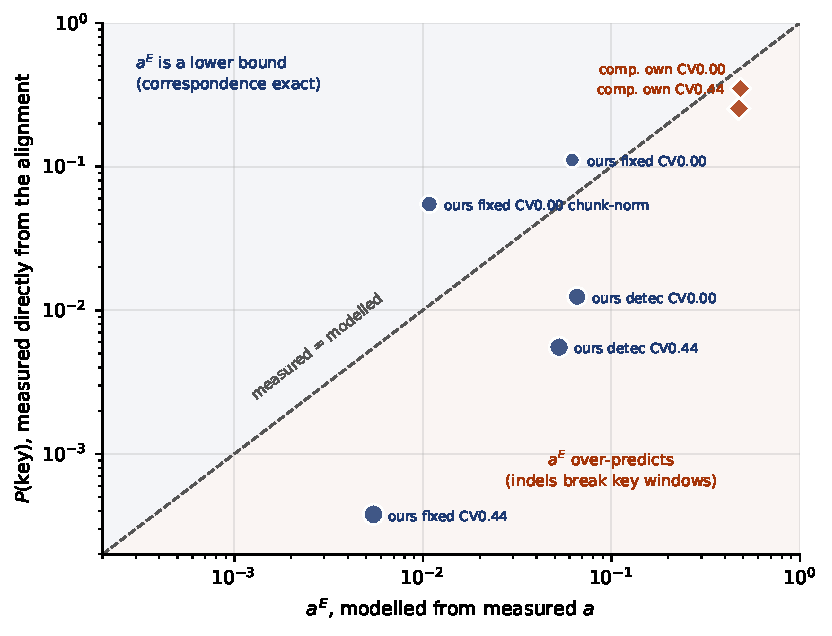
\includegraphics[width=0.66\textwidth]{fig7-3-model-vs-measured.pdf}
\caption{Measured key-match probability against the $a^{E}$ prediction, with marker area scaled
by the correspondence-failure rate $g$. $a^{E}$ is a lower bound only where correspondence is
exact.}
\label{fig:modelmeas}
\end{figure}

\section{Three root causes}
\label{sec:causes}

\subsection{Asymmetric event retention}

RawHash2~\cite{rawhash2} merges similar events: an event is dropped if its level differs
from the last retained
event by less than \texttt{--sig-diff} $=$ 0.35. The same rule is applied \textbf{to both the
reference encoding and the query}, and it keeps 73.4\% of events on each side. As a result, the
reference and the query contain the same number of events for any given span of signal.

Our pipeline does not have this property: its reference encoder outputs one event per $k$-mer,
while its query detector outputs about 0.78. Even at zero dwell dispersion, where there is no
timing noise, our indel rate is \textbf{0.170}. A rate this high
without noise indicates a structural mismatch between the two encoders, not a property of the
signal. Correspondence failure enters $P(\mathrm{key})$ with the same exponent as disagreement,
so it is just as costly. It is the first problem to fix, and fixing it needs a change to the
indexing path, not new research.

\subsection{A ${\approx}2.5$-bit quantisation sweet spot}

With a nominal four bits, RawHash2 could use sixteen buckets. On chr20, however, its symbols
fall into only six of them (7.7, 21.1, 9.7, 27.6, 24.0 and 8.8 per cent), plus 0.9 per cent in
an outlier bucket, giving a realised entropy of about \textbf{2.46 bits per event}. This is by
design: the quantiser is non-uniform, with fine resolution in a central band and coarse
resolution outside it.

A third system points the same way, which matters because two systems alone could agree by
coincidence.
Sigmoni~\cite{sigmoni}, which classifies rather than maps and shares none of our decision
machinery, quantises into an alphabet of \textbf{six} symbols by default---2.58 bits---on the
stated grounds that it balances robustness to noise against specificity in exact matching. Two
independent systems landing within a tenth of a bit of each other, one naming noise robustness
as the reason, suggests the operating point is not accidental.

Our uniform quantiser over a clipped $z$-range spends its alphabet evenly, realises more of it,
and agrees less. \textbf{The design axis is per-event entropy against per-event agreement, and
the two systems sit at opposite ends of it.} A key of 8 events at 2.46 bits carries about 19.7
bits of nominal specificity; one of 12 events at nearly 4 realised bits carries about 48. The
system with the \emph{less} specific key is five times more accurate, because specificity it
does not need costs it nothing and agreement it does need costs us everything.

\subsection{Recoverable loss inside the chainer}

The correspondence-aware measurement revises our frozen configuration's anchor supply from a
modelled 1.85 per read---derived from the simple $a^{E}$ form for a \emph{fixed-width}
configuration we do not ship---to a measured \textbf{14.9} for the configuration we do. The
observed median best-chain score is \textbf{4}.

So roughly 11 of 15 anchor-eligible positions per read are not reaching the best chain. This loss
was invisible while the estimate sat \emph{below} the observation: a decision stage cannot
recover more anchors than exist, and 1.85 against 4 left no room for loss. The candidates are the
occurrence cap discarding anchors before chaining, the 24-slot greedy chainer thrashing, and a
chaining band of 12 against a measured indel rate of 0.196. We have not isolated which.

\section{Discussion}
Our results lead to two recommendations.

\textbf{Measure $a$ and $g$ before designing a decision rule.} Both can be computed in a single
pass over paired reference and query events, without training or search, and together they show
whether \emph{any} decision rule can succeed before one is designed. A decision rule reported
without these figures cannot be assessed by the reader.

\textbf{Run the external baseline first, not last.} We evaluated every change to the decision
stage against our own earlier results, which varied by plausible amounts and never suggested
that the real limit lay elsewhere. A single run of a published tool on the same input
would have shown within a day that the gap was a factor of five, not a tuning problem. In an
ordered pipeline, internal improvements are measured against the wrong reference point until an
external baseline sets the scale.

\section{Limitations and threats to validity}
\label{sec:limits}

\textbf{All latency figures were measured under a hypervisor.} WSL2 can deschedule a vCPU
mid-decision, which in the data looks exactly like a slow decision. We therefore treat p50 and
p90 as properties of the implementation and p99 and above as upper bounds contaminated by the
platform. The direct evidence is the 2.0--59.4 ms spread of observed maxima, uncorrelated with
p99. A deadline-miss rate against the 1.56 ms bound requires bare metal with isolated
cores. We did not have it, and no claim here depends on the tail.

\textbf{All signal is simulated}, from two generators whose detector calibrations do not
transfer to each other by a factor of thirty, and every figure derives from a single
reference, human chr20. Agreement is measured at two dwell levels, one seed, 200 reads per
cell, where accuracy is swept at six levels in triplicate, so the claim that RawHash2's
agreement is dwell-invariant rests on two points. The alignment-based agreement figures are
upper bounds, computed under the correspondence that maximises matches; indel fractions of
0.055--0.208 mean the alignments are near-diagonal, so the estimator is not manufacturing
matches through heavy gapping, but the bound is one-sided and the asymmetry favours RawHash2.
The symmetric-retention explanation is visible in RawHash2's source and consistent with every
measurement, but the decisive ablation---applying our detector to our own reference encoding
and re-measuring---was not made. RawHash2, Squigulator, readfish and Icarust were built and
run here; claims about UNCALLED~\cite{uncalled}, Sigmap~\cite{sigmap},
RawAlign~\cite{rawalign} and Sigmoni~\cite{sigmoni} rest on their publications and
repositories rather than on execution.

\section{Conclusion}

We set out to determine whether the adaptive-sampling decision can be made in microseconds. It
can: a median of 124.8 \textmu{}s at genome scale against a 1.56 ms physical budget, with bounded
per-channel state, no allocation on the decision path, and no drops at the offered rate---while
the orchestration layer alone of a standard basecalling client costs 124.3 \textmu{}s per read-chunk
before any decision is made. The decision budget is not the obstacle to signal-space adaptive
sampling.

The question we answer better than the one we asked is why that is insufficient. Quantised-event
matching is bounded not by the rate at which decisions can be made but by the fidelity with which
signal survives segmentation and quantisation, captured by two measurable quantities whose
$E$-fold product governs everything downstream. At the agreement and correspondence our pipeline
achieves, no decision rule placed after quantisation can recover what segmentation and
quantisation discard---which is why six attempts to place one moved accuracy by at most 35\%
relative against a gap of a factor of five.

\section*{Reproducibility}

All code, data and scripts are in the accompanying repository at commit \texttt{eb0ea28}.
\texttt{scripts/verify\_paper\_numbers.py} recomputes every number in this paper from files
under \texttt{results/} and exits non-zero on any disagreement. Five claims are not settled by any
committed file and are documented as scope boundaries in the repository.

\begin{thebibliography}{10}

\bibitem{minknow} Oxford Nanopore Technologies: MinKNOW API,
\url{https://github.com/nanoporetech/minknow_api}

\bibitem{readfish} Payne, A., Holmes, N., Clarke, T., Munro, R., Debebe, B.J., Loose, M.:
Readfish enables targeted nanopore sequencing of gigabase-sized genomes. Nature Biotechnology
(2021)

\bibitem{uncalled} Kovaka, S., Fan, Y., Ni, B., Timp, W., Schatz, M.C.: Targeted nanopore
sequencing by real-time mapping of raw electrical signal with UNCALLED. Nature Biotechnology
(2021)

\bibitem{sigmap} Zhang, H., Li, H., Jain, C., Cheng, H., Au, K.F., Li, H., Aluru, S.: Real-time
mapping of nanopore raw signals. Bioinformatics 37(Suppl.~1) (2021)

\bibitem{rawhash} Firtina, C., Mansouri Ghiasi, N., Lindegger, J., Singh, G., Cavlak, M.B.,
Mao, H., Mutlu, O.: RawHash: enabling fast and accurate real-time analysis of raw nanopore
signals for large genomes. Bioinformatics 39(Suppl.~1) (2023)

\bibitem{rawhash2} Firtina, C., Soysal, M., Lindegger, J., Mutlu, O.: RawHash2: mapping raw
nanopore signals using hash-based seeding and adaptive quantization. arXiv:2309.05771 (2023)

\bibitem{rawalign} Lindegger, J., Firtina, C., Mansouri Ghiasi, N., Sadrosadati, M., Alser,
M., Mutlu, O.: RawAlign: accurate, fast, and scalable raw nanopore signal mapping via combining
seeding and alignment. arXiv:2310.05037 (2023)

\bibitem{sigmoni} Shivakumar, V., Ahmed, O., Kovaka, S., Zakeri, M., Langmead, B.: Sigmoni:
classification of nanopore signal with a compressed pangenome index. Bioinformatics (2024)

\bibitem{rawbench} Eris, M., Firtina, C., Mutlu, O., et al.: RawBench: a comprehensive
benchmarking framework for raw nanopore signal analysis techniques. In: ACM-BCB (2025).
arXiv:2510.03629

\bibitem{squigulator} Gamaarachchi, H., et al.: Squigulator: simulation of nanopore sequencing
signal data. Genome Research (2024)

\bibitem{icarust} Munro, R., Payne, A., Loose, M.: Icarust: a real-time simulator for nanopore
adaptive sampling, \url{https://github.com/LooseLab/Icarust}

\bibitem{misragries} Misra, J., Gries, D.: Finding repeated elements. Science of Computer
Programming 2(2) (1982)

\bibitem{spacesaving} Metwally, A., Agrawal, D., El Abbadi, A.: Efficient computation of
frequent and top-$k$ elements in data streams. In: ICDT (2005)

\bibitem{minimap2} Li, H.: Minimap2: pairwise alignment for nucleotide sequences.
Bioinformatics 34(18) (2018)

\bibitem{hdrhistogram} Tene, G.: HdrHistogram: a high dynamic range histogram,
\url{https://github.com/HdrHistogram/HdrHistogram_c}

\bibitem{minimizers} Roberts, M., Hayes, W., Hunt, B.R., Mount, S.M., Yorke, J.A.: Reducing
storage requirements for biological sequence comparison. Bioinformatics 20(18) (2004)

\end{thebibliography}

\end{document}
